\documentclass[mathserif,serif]{beamer}
\usetheme{Madrid}
\usecolortheme{seagull}
\beamertemplatenavigationsymbolsempty

\usepackage{graphicx}
\usepackage{listings}

\newenvironment{items}{
\begin{itemize}
  \setlength{\itemsep}{0pt}
  \setlength{\parskip}{7pt}
  \setlength{\parsep}{4pt}
}{\end{itemize}}

\begin{document}

\begin{frame}[t]
    \frametitle{About Me}

    \begin{items}
        \item Elvis Flesborg

        \item Master thesis on ITU Copenhagen
        \item Claus Brabrand as supervisor
        \item Jean Melo as co-supervisor
    \end{items}
\end{frame}

\begin{frame}[t]{About the Project}
    

    \begin{items}
        \item Make a representative sample of all configurations
        \item Look for errors in those configurations
        \begin{items}
            \item If too few are found, scale down to warnings
        \end{items}
    \end{items}

    
    Answer questions like:
    

    \begin{items}
        \item How many bugs are there in total?
        \item What types of bugs are there most of?
        \item Where are the bugs mostly located?
        \item \color{red}{... Any ideas?}
    \end{items}
\end{frame}

\begin{frame}[t]{About the Linux Kernel}
    

    \begin{items}
        \item 14172 different features \footnote{ grep -r "$\wedge\setminus$ *config\ " $|$ grep Kconfig $|$ awk -F':' '$\{$print \$ 2$\}$' $|$ sort $|$ uniq $|$ wc }.
        \item That is $2^{14172}$ different configurations minus invalid 
                configurations.
        \item Still more than estimated number of atoms in the known universe.
        \item Will use the already existing tool \emph{make randconfig}.
        \item Run 1 million times.
        \begin{items}
            \item Average compile time is 8 minutes
            \item 1 million times 8 minutes
            \item 55 computers
            \item 3 months
        \end{items}
    \end{items}
\end{frame}

\begin{frame}[t]
    
    \frametitle{The Sample}
    

    It is important to get a representative sample

    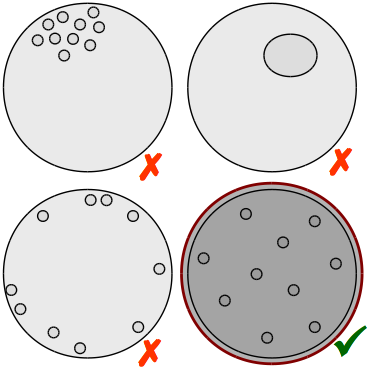
\includegraphics[scale=.5]{sample.png}
\end{frame}

\begin{frame}[t]{Compiling a Linux Kernel}

    \begin{items}
        \item `make randconfig` - create a random configuration.
        \item `make` - compile the Linux Kernel.
        \item Save all kinds of information about the compilation.
        \begin{items}
            \item Errors / warnings.
            \item Configuration.
        \end{items}
        \item Do it over and over again.
        \item Take cross-compiling into account.
    \end{items}


\end{frame}

\begin{frame}[t]{Kconfig}

    \begin{items}
        \item The language of the configurations.
        \begin{items}
            \item Data types
            \item Dependencies
            \item Menu structure (irrelevant to this project)
        \end{items}


    Example code, and explaination will be given.
    \end{items}
\end{frame}

\begin{frame}[t,fragile]{Kconfig - Grammar}
    \begin{lstlisting}
K ->      'config' ID TYPE OPTS
        | 'menuconfig' ID
        | 'if' ID K 'endif'
        | 'choice' K K+ 'endchoice'
        | 'menu' STRING K 'endmenu'

TYPE ->   'bool' | 'tristate' | 'string' | 'int'

OPTS ->   'default' STRING
        | 'help' STRING
        | 'range' INT
        | 'depends on' ID
        | 'select' ID
    \end{lstlisting}
\end{frame}

\begin{frame}[t,fragile]{Kconfig - Data types}
    \begin{columns}[T]
    \column{.5\textwidth}
    \begin{lstlisting}
config A
    bool
config B
    tristate
config C
    int
    range 5 15
config D
    hex
    default "c0000000"
config E
    string
    default "FOO"
    \end{lstlisting}
    \column{.5\textwidth}
    \begin{lstlisting}

yes, no (tristate)

yes, no, module

integers (string)


hexadecimals (string)


string
    \end{lstlisting}
    \end{columns}
\end{frame}

\begin{frame}[t,fragile]{Kconfig - Dependencies example}
    \begin{columns}[t]
    \column{.4\textwidth}
    \begin{lstlisting}
config A
    bool

config B
    bool
    depends on A

config C
    bool
    depends on A
    \end{lstlisting}

    \column{.2\textwidth}
    \textbf{Same as}

    \column{.4\textwidth}
    \begin{lstlisting}
config A
    bool

if A
    config B
        bool
    
    config C
        bool
endif
    \end{lstlisting}
    \end{columns}
\end{frame}

\begin{frame}[t,fragile]{Kconfig - Dependencies explaination}

    \begin{columns}[T]
    \column{.4\textwidth}
    \begin{lstlisting}
config A
    bool
    depends on B

config B
    bool
    depends on C

config C
    bool
    \end{lstlisting}
    \column{.6\textwidth}
    \begin{items}
        \item B can only be enabled if \emph{A} is enabled.
        \item `make randconfig` will roll a dice for the dependencies first.
        \begin{items}
            \item C, B, then A
        \end{items}
        \item Will not just autoselect \emph{A}. We have `select` for that.
    \end{items}

    \end{columns}
    
\end{frame}

\begin{frame}[t,fragile]{Kconfig - Select}

    \begin{columns}[T]
    \column{.4\textwidth}
    \begin{lstlisting}
config A
    bool
    select B

config B
    bool
    depends on C

config C
    bool
    \end{lstlisting}

    \column{.6\textwidth}

    \begin{items}
        \item \emph{select} forces the feature to be enabled without looking a 
                dependencies
        \item This will give and error in the case of $A \wedge  \neg C$
        \item In the Linux Kernel, they use pseudo-features to avoid problems.
    \end{items}

    \end{columns}
\end{frame}

\begin{frame}[t,fragile]{Kconfig - Pseudo-features}

    \begin{columns}[T]
    \column{.5\textwidth}

    \begin{lstlisting}
config A
    bool
    depends on D
    select HAVE_B
config HAVE_B
    bool
config B
    bool
    depends on HAVE_B && C

config C
    bool
config D
    bool
    \end{lstlisting}

    \column{.5\textwidth}

    \begin{items}
        \item If \emph{A} is enabled, it will force \emph{HAVE\_B} to be enabled
        \item \emph{HAVE\_B} does not have any dependencies that could break.
        \item This way, multiple features can force enable a dependency.
        \item No need for a `depends on A $\mid\mid$ B $\mid\mid$ C $\mid\mid$ D`
        \item The usual way to do it - but there are exceptions.
    \end{items}

    \end{columns}
\end{frame}

\begin{frame}[t,fragile]{Kconfig - Choice}

    \begin{columns}[T]
    \column{.4\textwidth}

    \begin{lstlisting}
choice
    prompt "Choose"
    default B
    depends on FOO

    config A
        bool
    config B
        bool
    config C
        bool

endchoice    
    \end{lstlisting}

    \column{.6\textwidth}

    \begin{items}
        \item Will only choose one of the features
        \begin{items}
            \item Unless it is a multiple-choice
            \item But I have only encountered one
            \item Plus - what's the point in those?
            \item Probably only visual
        \end{items}
        \item \emph{randconfig} counts the number of elements, and makes them 
                equally likely
        \item Inherit dependencies
        \item Default value
    \end{items}

    \end{columns}
\end{frame}

\begin{frame}[t,fragile]{Kconfig - Menu structure}

    \begin{columns}[T]
    \column{.5\textwidth}

    \begin{lstlisting}
menu "Letters"
    depends on ALPHABETH
    depends on !NUMBERS

    config A
        bool
    config B
        bool
endmenu

config ALPHABETH
    bool
config NUMBERS
    bool
    \end{lstlisting}

    \column{.5\textwidth}

    \begin{items}
        \item Gives dependencies to A and B
        \item Is for the visual representation
        \item \emph{randconfig} is not visual
        \item Also the \emph{comment} options is purely visual, and irrelevant to
                this project.
    \end{items}

    \end{columns}
\end{frame}

\begin{frame}[t,fragile]{randconfig bias}

    \begin{columns}[T]
    \column{.3\textwidth}

    \begin{lstlisting}
config A
    bool

config B
    bool
    depends on A

config C
    bool
    depends on B

config D
    bool
    depends on C
    \end{lstlisting}

    \column{.6\textwidth}

    \begin{items}
        \item Possible configurations with \emph{randconfigs} chances  are:
        \begin{items}
            \item () \emph{50\%}
            \item (A) \emph{50\%}
            \item (A,B) \emph{25\%}
            \item (A,B,C) \emph{12.5\%}
            \item (A,B,C,D) \emph{6.25\%}
        \end{items}
        \item This is biased, and not representative.
    \end{items}

    \end{columns}
\end{frame}

\begin{frame}[t,fragile]{randconfig bias 2}

    \begin{columns}[T]
    \column{.3\textwidth}

    \begin{lstlisting}
config A
    bool

config B
    bool
    depends on A

config C
    bool
    depends on B

config D
    bool
    depends on C
    \end{lstlisting}

    \column{.6\textwidth}

    \begin{items}
        \item We would prefer a totally equal chance:
        \begin{items}
            \item () \emph{20\%}
            \item (A) \emph{20\%}
            \item (A,B) \emph{20\%}
            \item (A,B,C) \emph{20\%}
            \item (A,B,C,D) \emph{20\%}
        \end{items}
    \end{items}

    \end{columns}
\end{frame}

\begin{frame}[t,fragile]{randconfig - elvisconfig}

    \begin{columns}[T]
    \column{0\textwidth}

    \begin{lstlisting}
    
    \end{lstlisting}

    \column{1\textwidth}

    \begin{items}
        \item Change \emph{randconfig} 
        \begin{items}
            \item Count the number of objects in the subtree.
            \item Change the randomness of the dice 
        \end{items}
        \item Create \emph{elvisconfig}
        \begin{items}
            \item Pick every feature value at random
            \item Do not look at dependencies
            \item Discard the invalid configurations
            \item Uniformly distributed
        \end{items}
        \item \color{red}{... Any ideas?}
    \end{items}

    \end{columns}
\end{frame}

\begin{frame}[t,fragile]{Threats to validity}

    \begin{columns}[T]
    \column{0\textwidth}

    \begin{lstlisting}
    
    \end{lstlisting}

    \column{1\textwidth}

    \begin{items}
        \item \emph{randconfig} being biased
        \item Not getting enough data
    \end{items}

    \end{columns}
\end{frame}


\begin{frame}[t,fragile]{Kconfig}

    \begin{columns}[T]
    \column{.4\textwidth}

    \begin{lstlisting}
    
    \end{lstlisting}

    \column{.6\textwidth}

    \begin{items}
        \item
    \end{items}

    \end{columns}
\end{frame}

extra if-example
config A
    bool " hej " if !B
(jeg tror nok, det er saadan det er)

randconfig vs. one-disabled

Threats to validity

The collected data.


\end{document}
